% F090｜给定直角边穷举勾股整数数组｜04_examples.tex
% 继承上传模板的 LaTeX 环境；当前条目的内容独立编写。
\clearpage
\begin{examplebox}
\textbf{\textcolor{CExample}{例 1：已知直角边9，找全}}
\par\medskip
\begin{center}
% F090｜pairs 原创简明教学示意图
\begin{tikzpicture}[>=stealth,scale=.94]
\node[draw,rounded corners,fill=teal!8] (a) at (0,0){$9^2=81$};
\node[draw,rounded corners,fill=orange!8,align=center] (b) at (4.2,0){$1\times81$\\$3\times27$\\$9\times9$};
\node[draw,rounded corners,fill=teal!13,align=center] (c) at (8.5,0){$(9,40,41)$\\$(9,12,15)$\\$b=0$ 排除};
\draw[->,thick] (a)--(b);\draw[->,thick] (b)--(c);
\end{tikzpicture}

\end{center}
\medskip
$81=1\times81=3\times27=9\times9$。第一对得 $b=40,c=41$；第二对得 $b=12,c=15$；第三对 $b=0$ 排除。答案 $(9,40,41),(9,12,15)$。
\end{examplebox}
\clearpage
\begin{examplebox}
\textbf{\textcolor{CExample}{例 2：已知直角边4，找全}}
\par\medskip
\begin{center}
% F090｜convert 原创简明教学示意图
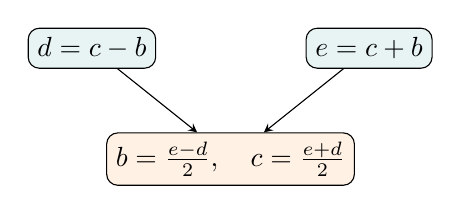
\begin{tikzpicture}[>=stealth,scale=.88]
\node[draw,fill=teal!9,rounded corners] (a) at (0,0){$d=c-b$};
\node[draw,fill=teal!9,rounded corners] (b) at (4,0){$e=c+b$};
\node[draw,fill=orange!10,rounded corners] (c) at (2,-1.6){$b=\frac{e-d}{2},\quad c=\frac{e+d}{2}$};
\draw[->] (a)--(c);\draw[->] (b)--(c);
\end{tikzpicture}

\end{center}
\medskip
$4^2=16$ 的正因数对为 $(1,16),(2,8),(4,4)$。第一对奇偶不同；第二对得 $b=3,c=5$；最后一对 $b=0$。所以只有 $\boxed{(3,4,5)}$。
\end{examplebox}
\clearpage
\begin{examplebox}
\textbf{\textcolor{CExample}{例 3：已知直角边6，找全}}
\par\medskip
\begin{center}
% F090｜parity 原创简明教学示意图
\begin{tikzpicture}[>=stealth,scale=.92]
\node[draw,rounded corners,fill=orange!8] at (0,0){$d,e$ 一奇一偶};
\node at (3.3,0){$\Rightarrow$};
\node[draw,rounded corners,fill=teal!9] at (7,0){$\frac{e-d}{2}$ 不是整数};
\node at (3.7,-1.2){\small 因数配对必须检查同奇同偶};
\end{tikzpicture}

\end{center}
\medskip
$36$ 的因数对 $(1,36),(2,18),(3,12),(4,9),(6,6)$。只有 $(2,18)$ 同偶且不相等，得 $b=8,c=10$，所以\textbf{只有} $(6,8,10)$。
\end{examplebox}
